% Created 2013-12-20 金 04:52
\documentclass[12pt]{jsarticle}
\usepackage[dvipdfmx]{graphicx}
\usepackage{comment}
%\usepackage{setspace}
%%\date{\today}
%\title{}
\textheight = 25truecm
\textwidth = 18truecm
\topmargin = -1.5truecm
\oddsidemargin = -1truecm
\evensidemargin = -1truecm
\marginparwidth = -1truecm
\def\theenumii{\Alph{enumii}}
\def\theenumiii{\alph{enumiii}}
\def\labelenumi{(\theenumi)}
\def\labelenumiii{(\theenumiii)}
%\setstretch{0.9}
\begin{document}

%\maketitle
%\tableofcontents

\begin{center}
%%%%%%%%%%%%%%%%%%%%%%%%%%%%%%%%%%%%%%%
%%%タイトル                         %%%
%%%%%%%%%%%%%%%%%%%%%%%%%%%%%%%%%%%%%%%
{\LARGE 受信バッファのアドレス決定の調査とその変更}
\end{center}

\begin{flushright}
  2014/12/12\\
  藤田将輝
\end{flushright}
%%%%%%%%%%%%%%%%%%1章%%%%%%%%%%%%%%%%%%%
\section{はじめに}
割り込み先OSの占有するコアがIPIを受信すると,
NICドライバが共有メモリからパケットを取得し,
割り込み処理をする割り込みハンドラを作成している.
割り込み処理において,受信バッファを特定する際,
どこから受信バッファのアドレスを参照し,
どの関数で受信バッファのアドレスを特定しているかを調査した.
また,受信バッファのアドレスをMintの共有メモリのアドレスに変更した.
本資料ではこの詳細を示す.

\section{最終目標と今回の変更}
本機構における最終目標について図1に示し,以下で説明する.
本機構の最終目標は以下の3つの機能により実現する.

\begin{itemize}
    \item[(機能1)] 共有メモリにパケットを格納する.
    \item[(機能2)] コア0にIPI送信要求を出し,コア0からコア1へIPIを送信する.
    \item[(機能3)] コア1がIPIを受信するとNICドライバが
        共有メモリからパケットを取得する.
\end{itemize}


\begin{figure}[ht]
    \begin{center}
        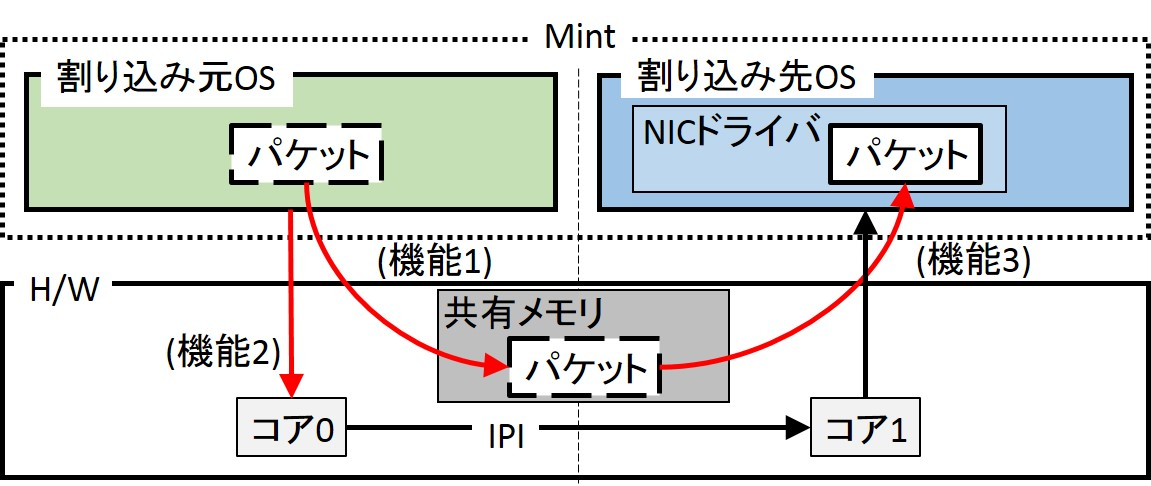
\includegraphics[height=5.0cm]{./fig1.jpg}
        \caption{最終目標}
        \label{fig1}
    \end{center}
\end{figure}

また,今回の改変を図2に示し,以下で説明する.
今回の改変により,以下の機能を実現する.


\begin{description}
    \item[(機能3’)] 共有メモリを参照可能になる.
\end{description}



\begin{figure}[t]
    \begin{center}
        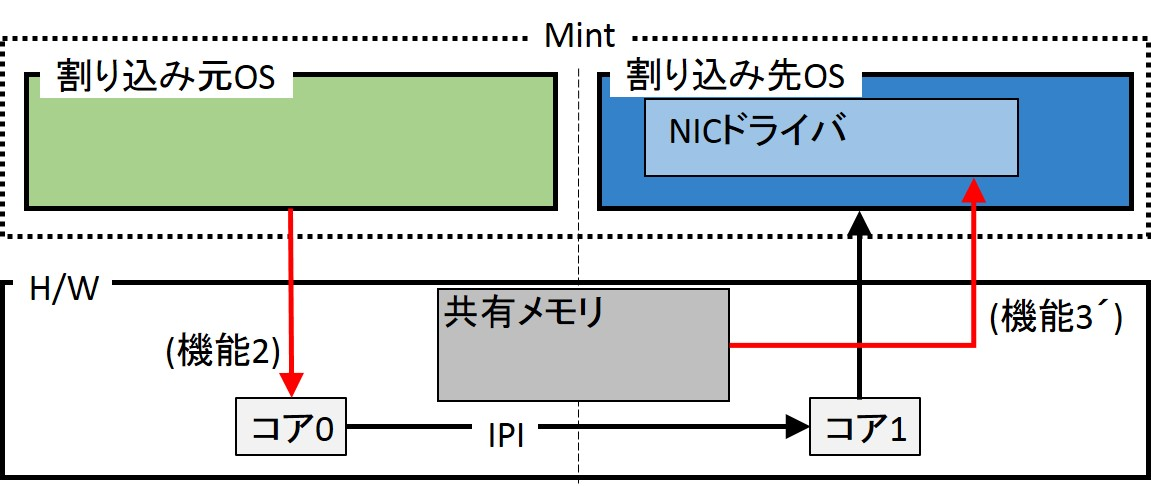
\includegraphics[height=5.0cm]{./fig2.jpg}
        \caption{改変}
        \label{fig2}
    \end{center}
\end{figure}

\section{受信バッファのアドレス}
受信バッファのアドレスはNICドライバのプライベート構造体である{\tt tp}
の受信ディスクリプタ{\tt RxDescArray}中の{\tt addr}に格納されている.
受信ディスクリプタとは受信バッファのアドレスや,受信状態の情報を保持している
ものである.
受信バッファは配列として定義されており,256個の要素を持っている.
この要素1つ1つが受信ディスクリプタを持っている.
次章では受信バッファのアドレスがどの関数内で受信ディスクリプタに格納されているかを示す.

\section{受信バッファのアドレス決定までの流れ}
% 受信バッファのアドレスは受信ディスクリプタの初期化を行う関数
% である{\tt rtl8169\_map\_to\_asic()}内で決定している.
% この{\tt rtl8169\_map\_to\_asic()}は受信バッファのアロケートを
% 行う関数{\tt rtl8169\_alloc\_rx\_data()}内で呼ばれており,
% 引数としてmappingという受信バッファのアドレスを渡している.
% また,受信バッファは配列として定義されており,各要素毎に
% 初期化処理を行なっている.
% 受信バッファに関する初期化処理をしているのが{\tt rtl8169\_rx\_fill()}
% である.
% この関数内で256個の要素すべてを初期化しており,
% {\tt rtl8169\_alloc\_rx\_data()}
% もここで呼ばれている.
% 以下にNICドライバの初期化処理の関数である{\tt rtl8169\_open()}が
% 実行されてから{\tt rtl8169\_map\_to\_asic()}が呼び出されるまでの流れを
% 以下に示す.
受信バッファの初期化を行い,受信ディスクリプタにアドレスが格納されるまでの流れを
以下に示す.
\begin{enumerate}
    \item {\tt rtl8169\_init\_ring()}\\
        受信バッファの初期化を行う関数である.
        受信バッファである{\tt Rx\_databuff}を初期化している.
        受信バッファを初期化すると{\tt rtl8169\_rx\_fill()}
        を呼び出す.
    \item {\tt rtl8169\_rx\_fill()} \\
        受信バッファのアロケートを行う関数である.
        配列として定義されている受信バッファの256個の要素全てをアロケートしている.
        アロケートをするためのデータを作成するために{\tt rtl8169\_alloc\_data()}
        を呼び出す.
    \item {\tt rtl8169\_alloc\_data()}\\
        受信バッファのアロケートを行うためのデータを作成する関数である.
        また,この関数で受信バッファのアドレスを決定し,{\tt rtl8169\_map\_to\_asic()}
        でそのアドレスをを格納する.
    \item {\tt rtl8169\_map\_to\_asic()}\\
        受信ディスクリプタにアドレスを格納する関数である.
        引数として受信バッファのアドレスをとり,これを受信ディスクリプタに格納する.
\end{enumerate}

次章では{\tt rtl8169\_alloc\_data()}を改変し,受信バッファのアドレスを
Mintの共有メモリのアドレスにしたときの詳細を示す.


\section{受信バッファのアドレスの変更}
受信バッファのアロケートを行うためのデータを作成する関数{\tt rtl8169\_alloc\_rx\_data()}内で,
{\tt rtl8169\_map\_to\_asic()}に受け渡す引数をMintの共有メモリのアドレスに変更した.
これにより,{\tt rtl8169\_map\_to\_asic()}内で,受信ディスクリプタである
{\tt RxDescArray}構造体の{\tt addr}に共有メモリのアドレスが格納される.
これにより,256個の受信ディスクリプタのアドレス全てを更新することができた.
また,アドレスの間隔は0x4000としている.
これは受信バッファのサイズが32KBのためである.
\section{確認}
アドレスを格納できていることを確認するため,
{\tt printk()}を用いて,256個の受信バッファのアドレスを表示させ,正しく格納できていることを
確認した.

\section{今後の課題}
今後の課題を以下に示す.

\begin{enumerate}
    \item パケットジェネレータの作成
    \item IPIにより動作し,共有メモリからパケットを取得する割り込みハンドラの作成
\end{enumerate}

\section{おわりに}
本資料では受信バッファの初期化と,これを用いて受信バッファのアドレスを
変更した際の詳細について述べた.
今後は課題を消化し,実装をすすめる.




\end{document}


